%%%%%%%%%%%%%%%%%%%%%%%%%%%
\chapter {Introduction}
\label{INTRO}
%%%%%%%%%%%%%%%%%%%%%%%%%%%

A distributed system is a group of computational entities cooperating with each other to achieve one or more tasks. This thesis deals with distributed computing by mobile agents in networks. More specifically, we deal with the problem of deploying a group of mobile agents that follow the same protocol,  to explore the network and decontaminate it from a dangerous virus (called Black Virus) present on some of the the network nodes.
In this Chapter, the motivations of the problem are provided, following is a brief summary of the contributions. 
Finally, an overview of the organization of the thesis is presented.


\section{Problem and Motivation} 
Mobile agents are widely used in distributed systems and networks. Their employ can cause some security issues, thus threatening   the network. For example, a contaminated or infected host can destroy working agents for various malicious purposes. A malicious agent can contaminate or infect other computer nodes so they become malfunctional or crashed.
  These static  harmful hosts, often called {\em Black Holes} (BH) trigger the problem called {\em Black Hole Search} (BHS), the focus of which is to locate their positions. This problem has been studied in several variants; in particular, in   different topologies, and under different assumptions on synchrony level   (synchronous vs. asynchronous). 
  Harmful agents trigger instead the problem called {\em Intruder Capture} (IC). The main focus of the Intruder Capture  is to deploy a group of mobile agents to capture an extraneous mobile agent (the intruder) that moves arbitrarily fast through the network and infects the visiting sites. Also this problem  has been investigated in a variety of topologies. A  detailed literature review will be provided in Chapter 2. Note that a black hole is static and   damages only  the agents reaching it without leaving any detectable trace. The intruder, instead,  is mobile and harmful to the network nodes, but does not cause any harm to other system agents. 
    A new harmful presence called {\em black virus} BV has been   introduced by Cai et al. in \cite{cai}. A BV is a dangerous process that resides at an unknown site in a network and destroys any upcoming agents, but unlike the BH, the node where the original BV resides   becomes clean when an agent reaches it. At the same time, the original BV multiplies, creating clones of itself, and spreads to all neighbouring nodes, thus increasing its presence and damage  in the network. A BV is destroyed when it moves to a site where there is already an agent. Based on this harmful presence, a new problem called {\em Black Virus Decontamination} (BVD) is presented by Cai et al., the main focus of which is to use a group of system agents to permanently remove any presence of the BV from the network. A protocol defining the actions of the agents solves the BVD problem if at least one agent survives and the network is free of BVs. Also, a desirable property of a  decontamination protocol is that the nodes which have been explored or cleaned by mobile agents are not   recontaminated by the BV spreading. A solution protocol with such a property is  called {\em monotone} (see \cite{monotone}).
Some important cost measures are: 
 the number of node infections by the BVs (casualties); 
the size of the team, i.e, the number of agents employed by the solution, and
the time needed by the solution. 
Solutions in which the agents explore the network's nodes sequentially have been proposed in \cite{alotaibi,cai,cai1} in various topologies. The size of the team is minimizes in \cite{cai,cai1} and the number of site infections is also minimized in such a case. However, in all those solutions, the time cost is quite high and not scalable, as it is linear in the size of the network.  In the thesis, we are interested in faster solutions using parallel strategies, where we deploy a larger number of mobile agents following the same protocol to decontaminate the network concurrently,  with the goal to  decrease time. For our strategies, we also introduce a new measure,   the {\em total working time} (TWT),  which is obtained as a combination of all three classical costs (number of agents,    execution time, casualties), and we compare it with the TWT of the existing algorithms.


%---------------------------------
\section{Our Contribution} 


\begin{enumerate}
\item In this thesis, we propose parallel strategies to solve the BVD problem. This is the first attempt to deal with this issue in a parallel way. Like in previous work, agents are not allowed to communicate with each other unless they are in the same network node so the protocol should enable the agents in different nodes to move independently but in  a synchronized fashion   to achieve the global goal.
We provide a simple   efficient solution to deal with this problem. 
%\color{blue} ? 
We also give the size of the minimum exploring team  to guarantee both the TWT and the  casualties we reach.  \color{black}
\item The BVD problem is investigated for three important topologies: {\em meshes}, {\em tori}, {\em chordal rings}. All the protocols are asymptotically optimal both in term of TWT and casualties. We compare our solutions with \cite{alotaibi} and  \cite{cai}, where the exploring route is  sequential, and the result is that our solution outperforms theirs in terms of both TWT and casualties. We  should   point out that in chordal rings especially, the more complicated the chordal ring becomes, the higher are the improvements of our algorithms in terms of in TWT  compared to \cite{alotaibi}.
\item The BVD problem is investigated also in the general case of the arbitrary topology. In this case we run extensive simulations to test its performance and we experimentally observe that also in this case, our solution is better than the existing sequential one.
\end{enumerate}

%---------------------------------

\section{Thesis Organization} 

The thesis is organized as follows:

Chapter 2 contains a literature review on related problems. We begin by reviewing the Black Hole Search and Intruder Capture problem, we then focus on the solution to the  BVD problem where the mobile agents explore the network sequentially. The problem has been studied in different topologies: two-dimensional grids, three-dimensional grids, tori, chordal rings, hypercubes and arbitrary network. Also, the variant of this problem, which is decontamination of an arbitrary network from multiple black virus, is   reviewed. 

Chapter 3 introduces terminology, definitions and model for the BVD problem used in the rest of the thesis.   We also describe the high level ideas that serve as the basis of all our solutions. Since monontonicity is a necessary condition for spread optimality, we explain this concept  and draw some  conclusions.

Chapter 4 focuses on the BVD problem for the mesh topology. In this chapter, an optimal algorithm in terms of casualties and TWT is developed. Complexity analysis  is performed and results obtained. Some comparisons  are also made between our solution and \cite{cai} and the result shows that our solution is better.

Chapter 5 presents the BVD problem for the chordal ring topology. In this chapter, we introduce the {\em Three Jump Notifying Technique} (TJNT) to manipulate each mobile agent to efficiently move along its route during the exploration,   and to avoid  the spread of clone BVs after the original BV is triggered. Based on this technique, we develop the parallel strategy for the mobile agents to decontaminate the chordal ring. Complexity analysis in terms of casualty and TWT are performed. Finally some comparisons are made between our solution and \cite{alotaibi} and the result shows that our solution performs better.

 
Chapter 6 proposes two parallel strategies to solve the BVD problem in the arbitrary graph: {\sc Flood} Strategy and {\sc Castle-First} Strategy. Flood Strategy completes the decontamination in $2d$ unit of time where $d$ is the diameter of the graph with a very high  cost  in terms of agents compared to any other   strategy; on the other hand,    the {\sc Castle-First} Strategy reaches a compromise between the sequential strategy and the {\sc Flood} Strategy: it employs  a reasonable number of agents and significantly less time than the sequential strategy.

 In Chapter 7, we experimentally study the BVD problem in the arbitrary graph. Details of simulation work are presented. We run experiments on different size of graphs with many connectivity densities and the results are collected and analyzed.
 

Chapter 8 summaries the main conclusion of our work and present some open problems and future work.
  



 \begin{comment}


\begin{figure}[H]
  \centering  
  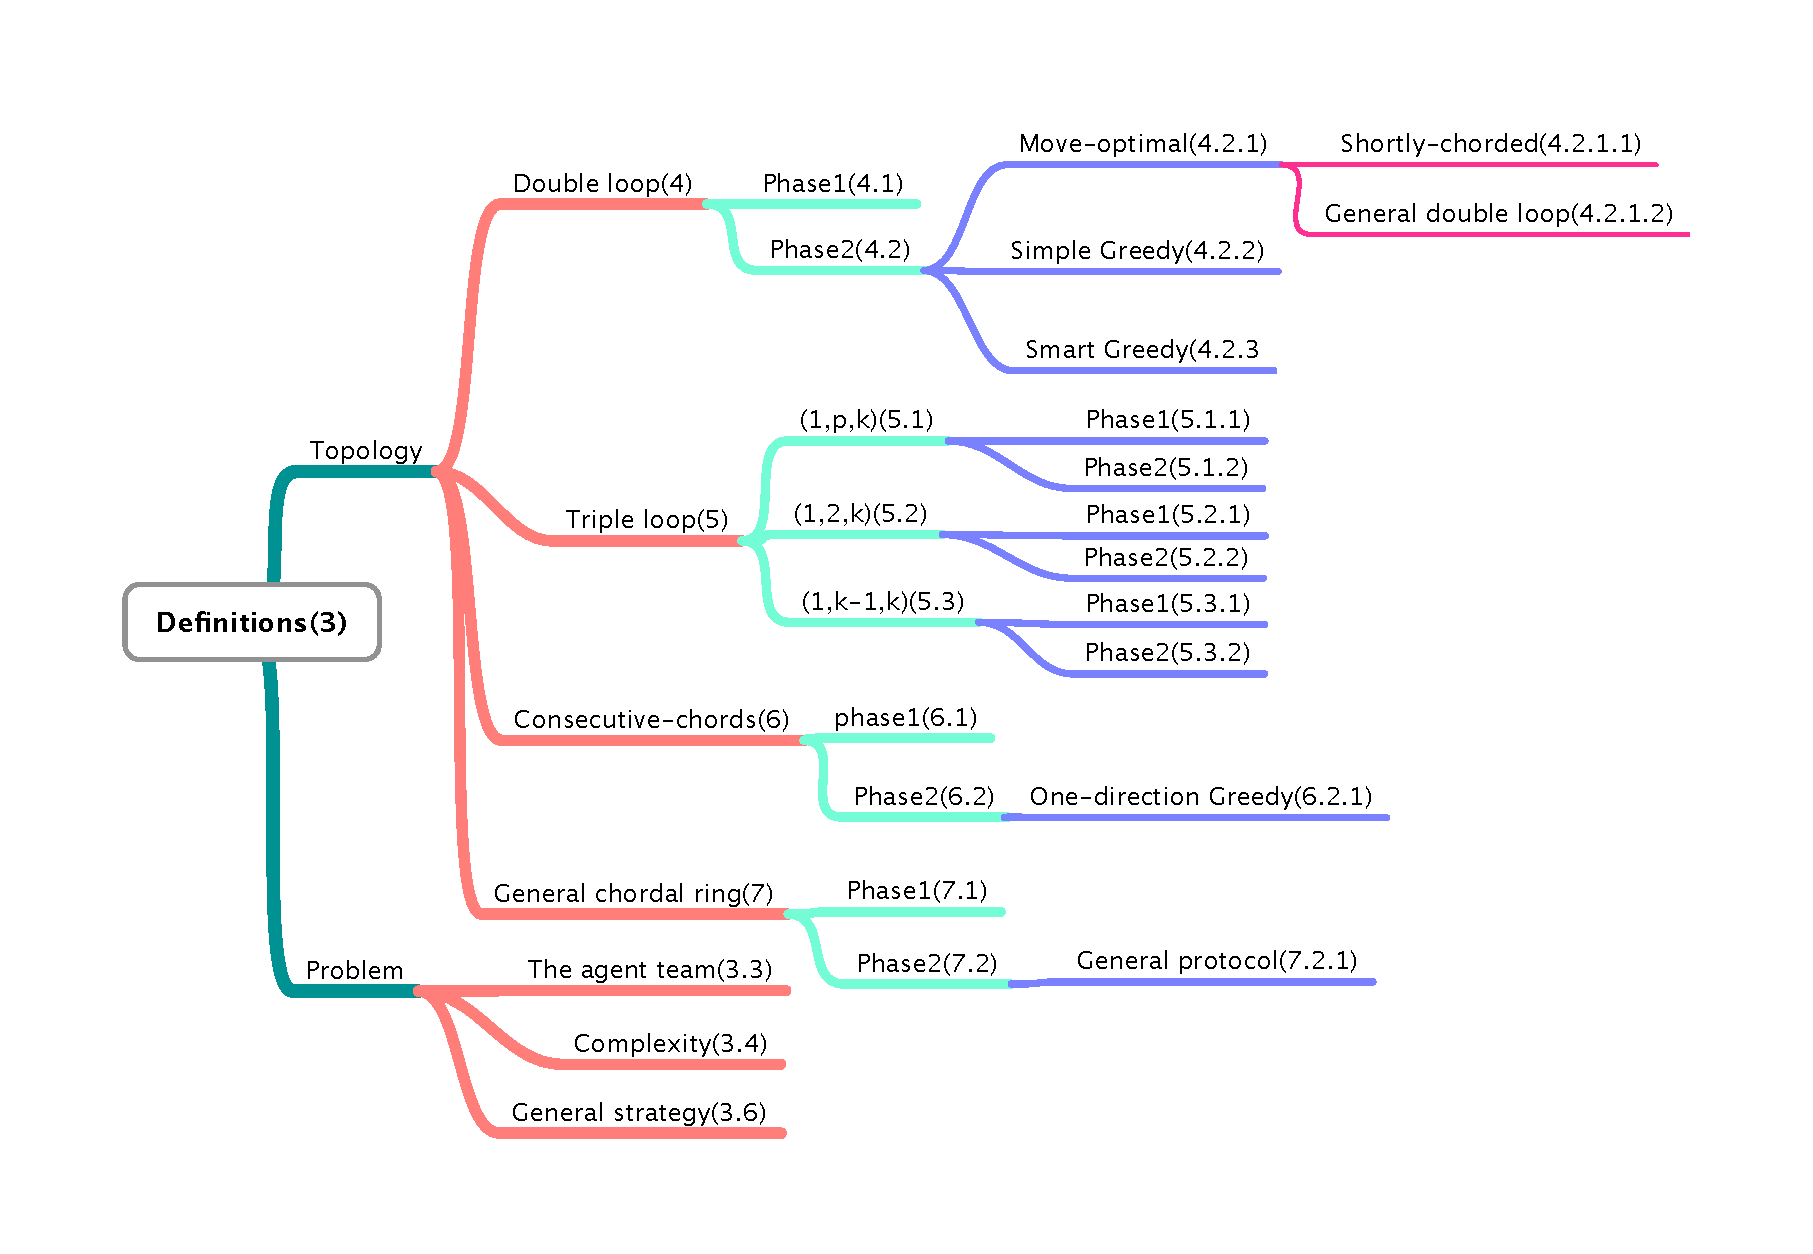
\includegraphics[width=1\textwidth]{figures/map2.pdf}
  \caption{A map showing the organization of the thesis}
\end{figure}

 \end{comment}
